%% ======================================================================
%% 03_description.tex -- 2. Hardware description (architecture, power, pins, decisions)
%% ======================================================================
\section{Hardware description}
\label{sec:description}

\subsection{Architecture}
Fig.~\ref{fig:overview} shows the final prototype and its CAD model, and Fig.~\ref{fig:architecture} shows its electrical and communications architecture. The robot is organized into four subsystems (three mechanical tiers and auxiliary electronics):

\begin{figure}[!htbp]
  \centering
  \begin{subfigure}[b]{0.43\textwidth}\centering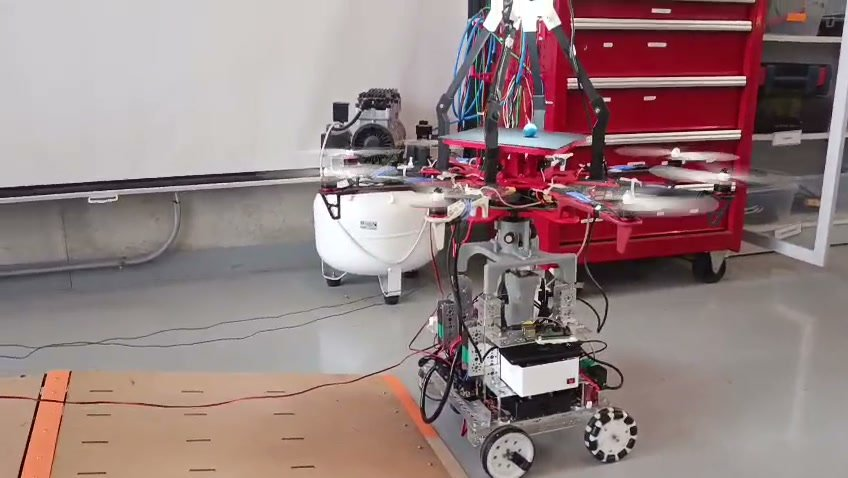
\includegraphics[width=\linewidth]{figures/photo_robot_side.jpg}\caption{Integrated prototype.}\end{subfigure}\hfill
  \begin{subfigure}[b]{0.30\textwidth}\centering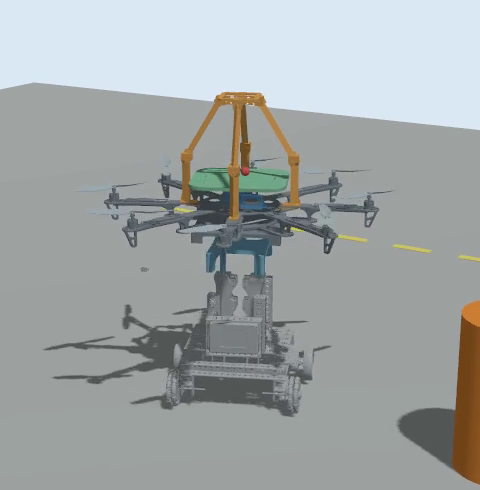
\includegraphics[width=\linewidth]{figures/cad_assembly.png}\caption{CAD assembly (383 parts).}\end{subfigure}\hfill
  \begin{subfigure}[b]{0.25\textwidth}\centering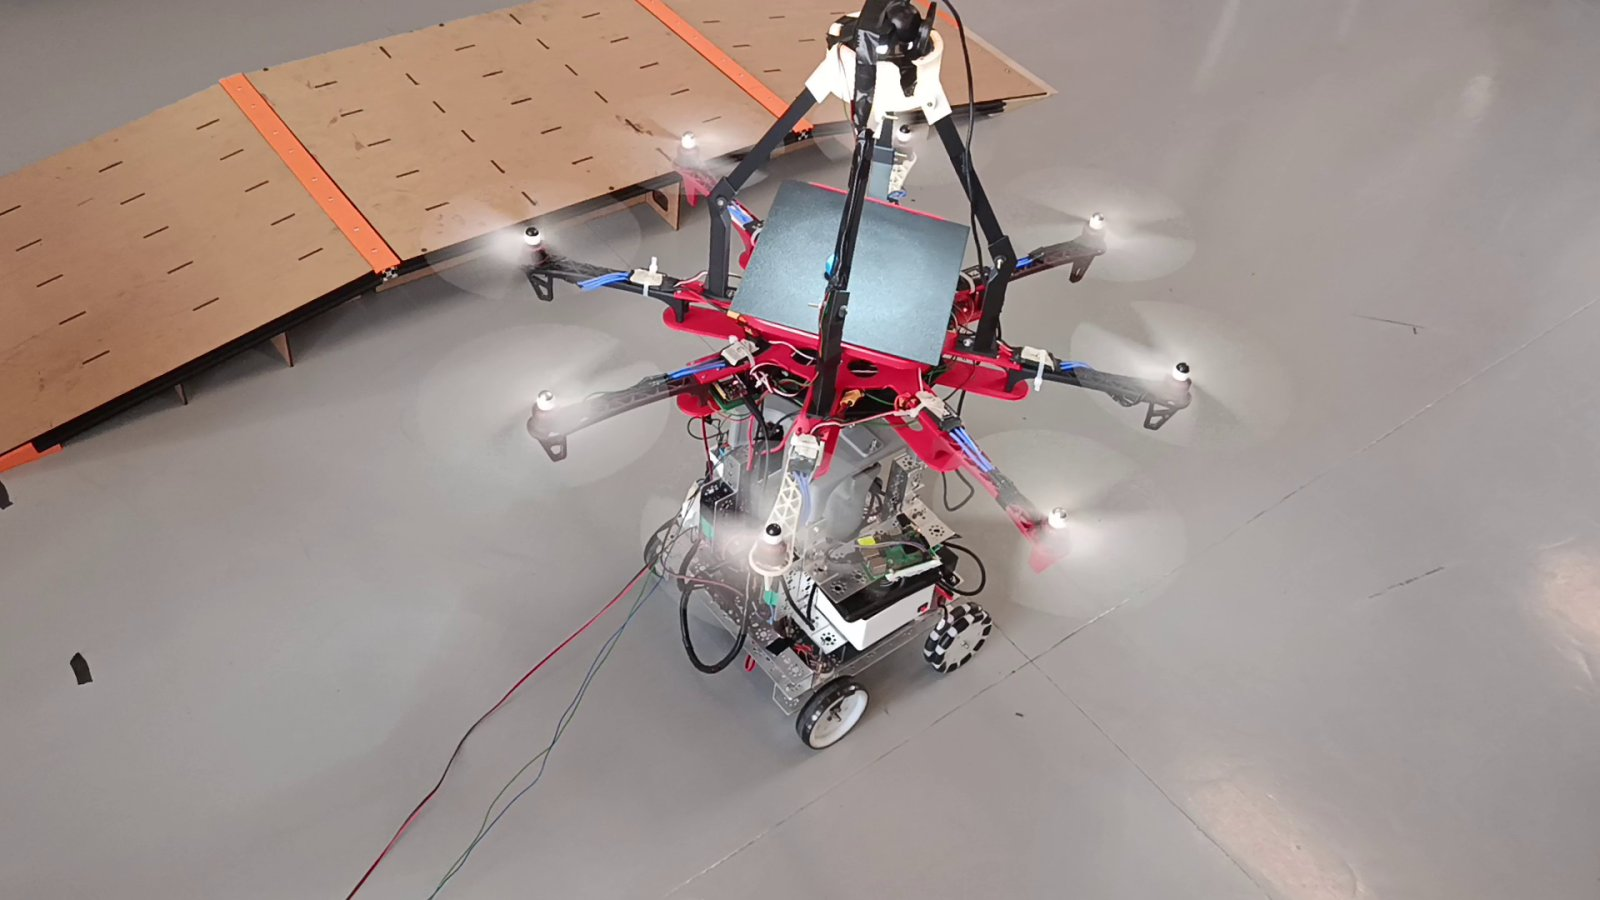
\includegraphics[width=\linewidth,trim=420 0 420 0,clip]{figures/photo_ramp_top.jpg}\caption{On the \SI{10}{\degree} ramp.}\end{subfigure}
  \caption{AeroTray. From bottom to top: TETRIX differential mobile base with myRIO, mast with vertical guide, spherical joint, octocopter (red frame, eight rotors), and ball-and-plate tray with overhead camera. The blue ball has a diameter of \SI{27}{\milli\metre}.}
  \label{fig:overview}
\end{figure}

\begin{enumerate}[label=\textbf{N\arabic*.}]
  \item \textbf{Mobile base.} TETRIX MAX aluminum chassis with two drive wheels (TETRIX TorqueNADO DC motors with quadrature encoders) and two omnidirectional wheels as passive supports. An NI myRIO-1900 reads the encoders, computes odometry, and executes a per-wheel PI velocity loop; an MDD10A H-bridge drives the motors from a \SI{12}{\volt} TETRIX NiMH battery. Track width $b=\SI{0.3794}{\metre}$; wheel travel per encoder count \SI{0.2151}{\milli\metre} (wheel radius $r\approx\SI{49.3}{\milli\metre}$).
  \item \textbf{Aerial module.} Octocopter with arms of radius $L=\SI{0.350}{\metre}$ (one motor every \SI{45}{\degree}), eight A2212 920\,KV brushless motors with 9450 propellers and 30\,A BEC-less ESCs, two 3S \SI{3300}{\milli\ampere\hour} LiPo batteries (one per group of four ESCs), an MPU-6050 IMU, and a VL53L0X time-of-flight sensor measuring distance to a matte-white target fixed to the base (Section~\ref{sec:altura}). A NodeMCU-32S (ESP32) runs attitude control at \SI{200}{\hertz}. The module mounts to the mast via a spherical joint on a carriage sliding along a vertical guide (measured travel of about \SI{140}{\milli\metre}); the spherical joint leaves roll and pitch free while friction and mechanical stops permit only a small yaw rotation, so the octocopter turns with the base. The moving assembly weighs \SI{3.6}{\kilo\gram} (\SI{3.3}{\kilo\gram} rotating assembly and \SI{0.3}{\kilo\gram} carriage). The rotor plane sits \SI{95}{\milli\metre} above the spherical joint center.
  \item \textbf{Ball-and-plate tray.} A $\SI{250}{\milli\metre}\times\SI{220}{\milli\metre}$ plate supported at its center on a universal joint atop a pillar fixed to the octocopter center plate, \SI{104}{\milli\metre} above the spherical joint, and tilted along two axes by two Futaba S3003 servos via four-bar linkages (Section~\ref{sec:linkage}). An ESP32-S3 generates the \SI{50}{\hertz} servo pulses (GPIO47 for $x$, GPIO21 for $y$) and runs the ball PID controller. A PS3 Eye camera, supported $\approx$\SI{0.20}{\metre} above the plate by four towers fixed to the octocopter (not the plate), streams $320\times240$ frames at \SI{187}{fps} to the Raspberry Pi, which detects the ball and sends its position and velocity to the ESP32-S3.
  \item \textbf{Supervisor, electronics distribution, and emergency stop.} The Raspberry Pi 3B+ centralizes vision, communications, and logging, with isolated logic domains and an emergency stop (Section~\ref{sec:power}). On the aerial module, both controllers mount beneath the center plate on opposite arms to balance weight and isolate ESC noise: the NodeMCU-32S (attitude control) on arm 8 ($+x$) and the ESP32-S3 (tray) on arm 6 ($-x$). The MPU-6050 IMU and VL53L0X laser sit beside the NodeMCU on arm 8 on the same I$^2$C bus, with the laser pointing down at the fixed target on the base. Both sensors are therefore offset from the spherical joint axis, and Section~\ref{sec:altura} corrects the height measurement for this lever arm.
\end{enumerate}

\begin{figure}[!htbp]
\centering
\begin{tikzpicture}[font=\footnotesize, >=Latex,
  colhdr/.style={font=\footnotesize\bfseries, text=pGris!85!black, align=center},
  blk/.style={draw, rounded corners=2pt, align=center, minimum height=11.5mm, inner xsep=2pt, inner ysep=2.5pt, line width=0.6pt},
  blkusr/.style={blk, fill=white, draw=pGris, text width=3.34cm},
  blkpw/.style={blk, fill=pRojo!7, draw=pRojo, text width=3.34cm},
  blkcp/.style={blk, fill=pAzul!7, draw=pAzul, text width=3.34cm},
  blksa/.style={blk, fill=pVerde!7, draw=pVerde, text width=4.04cm},
  pw/.style={->, line width=1.05pt, pRojo, rounded corners=2pt},
  pwbr/.style={pw, preaction={-, draw=white, line width=2.6pt, rounded corners=2pt}},
  dt/.style={<->, line width=0.85pt, pAzul, rounded corners=2pt},
  dt1/.style={->, line width=0.85pt, pAzul, rounded corners=2pt},
  lab/.style={font=\footnotesize, text=pAzul!90!black, inner sep=1.5pt}]
  % 3-column coordinates (total width = 13.38 cm < 13.74 cm = \textwidth)
  % Col 1: x=1.74 ([0.00, 3.48]), Col 2: x=6.28 ([4.54, 8.02]), Col 3: x=11.24 ([9.15, 13.33])
  \node[colhdr] at (1.74, -0.84) {Power};
  \node[colhdr] at (6.28, 0.90) {Compute};
  \node[colhdr] at (11.24, 0.90) {Sensors and actuators};

  % ---- Row 1 (y = 0.00) -- all boxes exactly 2 lines and equal height
  \node[blkusr] (web)  at (1.74,  0.00) {\textbf{Web browser}\\ laptop or phone};
  \node[blkcp]  (pi)   at (6.28,  0.00) {\textbf{Raspberry Pi 3B+}\\ vision, logging, web};
  \node[blksa]  (cam)  at (11.24, 0.00) {\textbf{PS3 Eye camera}\\ 320$\times$240 at 187 fps};

  % ---- Row 2 (y = -1.68)
  \node[blkpw]  (pipw) at (1.74, -1.68) {\textbf{BT5: 3S 18650}\\ XL4015 $\to$ 5.2 V};
  \node[blkcp]  (s3)   at (6.28, -1.68) {\textbf{ESP32-S3}\\ ball PID};
  \node[blksa]  (srv)  at (11.24,-1.68) {\textbf{2$\times$ Futaba S3003}\\ tray servos};

  % ---- Row 3 (y = -3.36)
  \node[blkpw]  (bt6)  at (1.74, -3.36) {\textbf{BT6: 3S 18650}\\ 5.2 V (servos, SB1)};
  \node[blksa]  (imu)  at (11.24,-3.36) {\textbf{MPU-6050, VL53L0X}\\ IMU and height laser};

  % ---- Row 4 (y = -5.04)
  \node[blkpw]  (lipo) at (1.74, -5.04) {\textbf{2$\times$ LiPo 3S}\\ 30 A fuses, K1, K2};
  \node[blkcp]  (nm)   at (6.28, -5.04) {\textbf{NodeMCU-32S}\\ attitude at 200 Hz};
  \node[blksa]  (esc)  at (11.24,-5.04) {\textbf{8$\times$ 30 A ESCs}\\ and drone motors};

  % ---- Row 5 (y = -7.08)
  \node[blkpw]  (bt4)  at (1.74, -7.08) {\textbf{BT4: power bank}\\ 5 V $\to$ 12 V boost};
  \node[blkcp]  (rio)  at (6.28, -7.08) {\textbf{NI myRIO-1900}\\ odometry, PI loop};
  \node[blksa]  (hb)   at (11.24,-7.08) {\textbf{MDD10A H-bridge}\\ 2$\times$TorqueNADO, enc.};

  % ---- Row 6 (y = -8.68)
  \node[blkpw]  (nimh) at (1.74, -8.68) {\textbf{12 V NiMH}\\ TETRIX, 20 A, K3};

  % ---- Data links (blue #0072B2)
  \draw[dt]  ([yshift=2.2mm]web.east) -- node[lab, above=1.5pt]{Wi-Fi} ([yshift=2.2mm]pi.west);
  \draw[dt]  (pi.east) -- node[lab, above=1.5pt]{USB} (cam.west);
  \draw[dt]  ([xshift=3mm]pi.south) -- node[lab, right=2pt]{USB} ([xshift=3mm]s3.north);
  \draw[dt1] (s3.east) -- node[lab, above=1.5pt]{PWM} (srv.west);

  % Pi <-> NodeMCU (USB) via left corridor of Col 2 and open Row 3 cell
  \draw[dt] ([xshift=-9mm]pi.south) -- ++(0,-0.42) -| (4.35,-3.36)
            -- node[lab, above=1.5pt, pos=0.55]{USB} (6.28,-3.36) -- (nm.north);
  % Pi <-> myRIO (UART 9600) via parallel corridor and open lane above myRIO
  \draw[dt] ([xshift=-13mm]pi.south) -- ++(0,-0.20) -| (3.98,-6.24)
            -- node[lab, above=1.5pt, pos=0.60]{UART 9600} (6.28,-6.24) -- (rio.north);

  % NodeMCU <-> IMU+VL53 (I2C) and NodeMCU -> ESC (PWM)
  \draw[dt]  ([xshift=10mm]nm.north) |- (8.05,-3.36) -- node[lab, above=1.5pt]{I$^2$C} (imu.west);
  \draw[dt1] (nm.east) -- node[lab, above=1.5pt]{PWM} (esc.west);
  % myRIO <-> MDD10A+TorqueNADO (PWM and encoders)
  \draw[dt1] ([yshift=2mm]rio.east) -- node[lab, above=1.5pt]{PWM} ([yshift=2mm]hb.west);
  \draw[dt1] ([yshift=-2mm]hb.west) -- node[lab, below=1.5pt]{enc.} ([yshift=-2mm]rio.east);

  % ---- Power links (red #D55E00)
  \draw[pw]   (pipw.east) -- (3.72,-1.68) |- ([yshift=-2.4mm]pi.west);
  \draw[pwbr] (bt6.east)  -- (3.72,-3.36) |- (3.72,-2.52) -| (srv.south);
  \draw[pwbr] (lipo.east) -- (3.72,-5.04) |- (3.72,-5.82) -| (esc.south);
  \draw[pw]   (bt4.east)  -- (rio.west);
  \draw[pw]   (nimh.east) -| (hb.south);

  % ---- Legend inside figure (centered below Row 6)
  \node[draw=pGris!60, rounded corners=2pt, fill=white, inner xsep=6pt, inner ysep=4pt, anchor=north]
    (leg) at (6.66,-9.48) {%
    \begin{tikzpicture}[baseline=-0.5ex, font=\footnotesize]
      \draw[dt]  (0.00,0) -- (0.58,0); \node[right=2.5pt, inner sep=0pt] at (0.58,0) {Data};
      \draw[pw]  (1.75,0) -- (2.33,0); \node[right=2.5pt, inner sep=0pt] at (2.33,0) {Power};
      \draw[fill=pRojo!7,  draw=pRojo,  rounded corners=1pt] (3.70,-0.12) rectangle (4.00,0.12);
      \node[right=2.5pt, inner sep=0pt] at (4.00,0) {Supplies};
      \draw[fill=pAzul!7,  draw=pAzul,  rounded corners=1pt] (5.70,-0.12) rectangle (6.00,0.12);
      \node[right=2.5pt, inner sep=0pt] at (6.00,0) {Compute};
      \draw[fill=pVerde!7, draw=pVerde, rounded corners=1pt] (7.82,-0.12) rectangle (8.12,0.12);
      \node[right=2.5pt, inner sep=0pt] at (8.12,0) {Sensors and actuators};
    \end{tikzpicture}};
\end{tikzpicture}
\caption{Electrical and communications architecture. Power domains share ground only through signal cables; the Raspberry Pi powers the camera, ESP32-S3, and NodeMCU-32S over USB. Pin assignments are listed in Table~\ref{tab:pins} and message frames in Section~\ref{sec:interfaces}.}
\label{fig:architecture}
\end{figure}

\subsection{Power system and emergency stop}
\label{sec:power}
Power distribution follows the Rev.~I electrical schematic (18 Nov 2026), released with the design files, and the group's power audit. Five independent power domains connect only through the signal grounds of the PWM and USB cables:
\begin{enumerate}[label=\textbf{S\arabic*.}]
  \item \textbf{Drone propulsion, two isolated branches.} Each 3S \SI{3300}{\milli\ampere\hour} 25C LiPo battery (BT1, BT2) runs through an XT60 connector, a \SI{30}{\ampere} ATO fuse (F1, F2), and contacts 30--87 of an automotive relay (K1, K2), then up to the drone via an $\approx$\SI{1}{\metre} 14\,AWG cable (loop resistance \SI{16.6}{\milli\ohm}) to a \SI{1000}{\micro\farad}/\SI{25}{\volt} capacitor per node. Branch A supplies ESCs 1, 3, 5, and 7 (M1, M3, M5, M7), and branch B supplies ESCs 2, 4, 6, and 8. Each branch drives two opposing pairs with two motors of each rotation direction, so an unevenly discharged battery lowers total thrust without producing yaw torque. Negative rails A$-$ and B$-$ join only on the drone (GND\_D), and the red BEC wire of every ESC is cut.
  \item \textbf{TETRIX base.} A \SI{12}{\volt} \SI{3000}{\milli\ampere\hour} NiMH pack (BT3), internal \SI{20}{\ampere} fuse, and relay K3 feed the MDD10A H-bridge ($2\times\SI{10}{\ampere}$) and both TorqueNADO motors.
  \item \textbf{myRIO.} A \SI{5}{\volt}/\SI{3}{\ampere} power bank (BT4) and a 5-to-\SI{12}{\volt} boost converter supply the myRIO, which powers the encoders.
  \item \textbf{\SI{5}{\volt} logic} (root of the ground tree). A 3S 18650 pack with BMS (BT5), \SI{3}{\ampere} fuse, switch SW1, and XL4015 regulator set to \SI{5.2}{\volt} powers the Raspberry Pi and, through the USB hub, the NodeMCU-32S (with its sensors) and the ESP32-S3.
  \item \textbf{Servos and emergency stop.} A second 3S 18650 pack with BMS (BT6), \SI{3}{\ampere} fuse, SW2, and XL4015 feeds both S3003 servos (with \SI{1000}{\micro\farad} and $2\times\SI{100}{\micro\farad}$ capacitors) and the LED ring. Through a \SI{1}{\ampere} fuse and a \SI{4}{\metre} two-conductor cable, the same pack energizes relay coils K1--K4 via the latching normally closed mushroom emergency stop (SB1) on the control box; each coil carries a 1N4007 flyback diode. Pressing SB1 simultaneously opens both LiPo branches, the base battery, and servo power (K4), while logic remains powered and logging.
\end{enumerate}
In hover, each branch delivers 18--\SI{22}{\ampere} (60--75\% of the fuse rating; Section~\ref{sec:bateria}). Above \SI{1850}{\micro\second}, current approaches \SI{30}{\ampere}, so the firmware restricts operation in that band to \SI{20}{\second}. The Rev.~I schematic omits battery sensing: although the Rev.~E wiring diagram shows \SI{10}{\kilo\ohm}/\SI{3.3}{\kilo\ohm} dividers to GPIO34 and GPIO35, firmware v11 does not read them, and LiPo voltages are measured manually before and after each session (Section~\ref{sec:operation}).

\subsection{Pin assignments}
\label{sec:pins}
Some earlier project documents (previous wiring diagrams and the power audit's proposal to relocate ESC4 and ESC7) diverge from the code. Table~\ref{tab:pins} follows the flight firmware released in \fn{03_firmware}.

\begin{table}[!htbp]
\centering
\caption{Embedded controller pin assignments per the flight firmware: drone v11 and ESP32-S3 ball PID (folder \texttt{03\_firmware}).}
\label{tab:pins}
\small
\begin{tabularx}{\textwidth}{@{}llX@{}}
\toprule
Controller & Pin & Function \\
\midrule
NodeMCU-32S (U10) & GPIO25, 27, 21, 5 & \SI{50}{\hertz} PWM for M1, M3, M5, M7 (branch A) \\
 & GPIO26, 14, 19, 17 & \SI{50}{\hertz} PWM for M2, M4, M6, M8 (branch B) \\
 & GPIO23 / GPIO22 & I$^2$C SDA / SCL at \SI{100}{\kilo\hertz}: MPU-6050 (0x68) and VL53L0X (0x29) \\
 & GPIO34 / GPIO35 & VBAT\_A / VBAT\_B via $\div4.03$ divider (wired in Rev.~E; unused by firmware v11) \\
 & USB & \SI{5}{\volt}, commands, heartbeat, and telemetry with the Raspberry Pi \\
ESP32-S3 (U16) & GPIO47 / GPIO21 & $x$-servo / $y$-servo pulse (\SI{50}{\hertz}, neutral 1386/\SI{1392}{\micro\second}, $\pm\SI{220}{\micro\second}$) \\
Raspberry Pi 3B+ & GPIO14 / GPIO15 & UART TX / RX to myRIO MXP-A pin 10 (RX) / pin 14 (TX), 9600 8N1 \\
myRIO-1900 & MXP-A, MXP-B & PWM and DIR to MDD10A and encoder inputs (left motor on MXP-A, right on MXP-B); UART on MXP-A \\
\bottomrule
\end{tabularx}
\end{table}

GPIO5 and GPIO14 output glitch pulses during ESP32 boot. As long as ESCs remain on those pins, the LiPo branches are energized (releasing SB1 to close K1 and K2) only after the NodeMCU has booted and is outputting \SI{1000}{\micro\second} to all ESCs.

\subsection{Supervisor and interfaces}
\label{sec:interfaces}
The Raspberry Pi 3B+ serves as the system hub. Its program (\texttt{seguidor.py}) performs five functions:
\begin{itemize}
  \item captures raw YUYV frames from the PS3 Eye at \SI{187}{fps}, rectifies the plate with a four-corner homography, and detects the ball by color with OpenCV \cite{bradski2000};
  \item streams ball position and velocity to the ESP32-S3 over USB serial (frame \texttt{p x,y,vx,vy});
  \item exchanges commands, a heartbeat (\texttt{hb}), and telemetry with the octocopter over USB serial;
  \item communicates with the myRIO over the hardware UART on the GPIO header;
  \item logs all streams to CSV files and serves three web pages: \texttt{/} (ball and plate), \texttt{/dron} (octocopter), and \texttt{/robot} (full robot).
\end{itemize}
The myRIO and Pi exchange two text frames at 9600\,baud, 8N1:
\begin{itemize}
  \item from myRIO to Pi, \texttt{cmd1,cmd2}, where codes 1--4 command the octocopter and codes 5--11 command the ball-and-plate stage;
  \item from Pi to myRIO, every \SI{50}{\milli\second}, \texttt{x,y,roll,pitch,uav,bp}.
\end{itemize}
Commands received from the myRIO take priority over web commands for \SI{250}{\milli\second}.

\subsection{Design decisions and modifications}
The final configuration emerged from several iterations; the key decisions are:
\begin{itemize}
  \item \textbf{A drone rather than a gimbal on the base.} The octocopter fulfills two roles a motorized gimbal cannot achieve simultaneously: it levels relative to gravity, eliminating ground slope from the ball dynamics (Section~\ref{sec:chain}), and it supports part of its own weight, lowering the robot's effective center of mass on a ramp and reducing climbing torque (Section~\ref{sec:porquedron}).
  \item \textbf{Passive spherical joint instead of free flight.} A spherical joint on a vertical guide allows the octocopter to balance in roll and pitch and lift a few centimeters while remaining captive; this ensures indoor safety and preserves the mechanical base coupling under study.
  \item \textbf{Eight rotors.} With 8 motors, the \SI{3.6}{\kilo\gram} assembly hovers on charged batteries at 1725--\SI{1775}{\micro\second} (68--74\% of the usable map range), allowing the mixer to trade collective thrust for attitude torque (Section~\ref{sec:aerial}). Thrust margin depends strongly on battery voltage (Section~\ref{sec:bateria}).
  \item \textbf{Camera on the Pi instead of on the ESP32.} The first version used a camera on the ESP32-S3, limited to about 50\,fps by JPEG compression (lowering JPEG quality caused hundreds of corrupt frames per minute). Switching to a PS3 Eye on the Pi raised the rate to \SI{187}{fps} with uncompressed frames, making velocity estimation and the ball PID derivative term usable; remaining loop delay sets the derivative-gain ceiling (Section~\ref{sec:ballcontrol}).
  \item \textbf{Isolated power domains.} Each subsystem has its own supply and domains share only ground (Section~\ref{sec:power}). The original BMS for servos and relay coils failed during testing and was replaced by a bench supply in part of the trials (Section~\ref{sec:limits}).
  \item \textbf{Flight firmware iterations.} Nine guided-flight trials led to firmware v9 (Section~\ref{sec:flights}): an accelerometer low-pass filter against rotor vibration, an active yaw loop, a larger angle-integral term, a wider in-flight angular-rate command limit, and hysteresis in flight-gain switching. The model in Section~\ref{sec:authority} explains why the decisive change was the angular-rate command limit rather than the gains. The final v11 release added a sliding yaw window at idle for base turns and a Kalman filter with cascaded altitude control over the calibrated laser (Section~\ref{sec:altura}).
\end{itemize}
